\documentclass{standalone}
\usepackage{tikz, pgfmath}
\usetikzlibrary{calc}


% draw stack of mapped reads
%
% Parameters
% #1: SNP coordinate on reference genome
% #2: number of reads
% #3: + or - depending on the direction to grow the stack (up or down, respectively)
% #3: + or - depending on small baseline correction to avoid reads overlap at neighboring SNPs (up or down, respectively)
% #5: style of the read
% #6: style of the SNP variant on the read
\newcommand{\mappedreads}[6]{
\path (#1) ++(0, #3 5pt) ++(0, #4 0.75pt) coordinate (baseline);
\draw[#5] let \n1 = {0.2} in foreach \y in {1,...,#2} { (baseline) ++(0, \y * #3 3pt) node[#6] {} ++(rand * \n1, 0) +(-\n1,0) -- +(\n1,0) };
}

% draw genome 1
%
% Parameters
% #1: style of DNA
% #2: vertical position
% #3-6: style of SNP variants
\newcommand{\genomeone}[6]{
\coordinate (horiz) at (0,#2);
\path (horiz) ++(0,3pt) coordinate (geneupperedge);
\path[orf] (g1g1start|-horiz) ++(0,-3pt) rectangle (g1g1end|-geneupperedge);
\path[orf] (g1g2start|-horiz) ++(0,-3pt) rectangle (g1g2end|-geneupperedge);
\draw[#1] (g1start|-horiz) -- (g1g1s1|-horiz) node[#3] {} -- (g1g1s2|-horiz) node[#4] {} -- (g1g1s3|-horiz) node[#5] {} -- (g1g2s1|-horiz) node[#6] {} -- (g1end|-horiz);
}

\newcommand{\genometwo}[6]{
\coordinate (horiz) at (0,#2);
\path (horiz) ++(0,3pt) coordinate (geneupperedge);
\path[orf] (g2g1start|-horiz) ++(0,-3pt) rectangle (g2g1end|-geneupperedge);
\path[orf] (g2g2start|-horiz) ++(0,-3pt) rectangle (g2g2end|-geneupperedge);
\draw[#1] (g2start|-horiz) -- (g2g1s1|-horiz) node[#3] {} -- (g2g1s2|-horiz) node[#4] {} -- (g2g1s3|-horiz) node[#5] {} -- (g2g2s1|-horiz) node[#6] {} -- (g2end|-horiz);
}


\newcommand{\matRNAgenomeone}[7]{
\coordinate (horiz) at (0,#1);
\foreach \y in {1,...,#6} {
\path (horiz) +(0, \y * 3pt) coordinate (hrz);
\draw[matread]
(g1g1start|-hrz) -- (g1g1s1|-hrz) node[#2] {} -- (g1g1s2|-hrz) node[#3] {} -- (g1g1s3|-hrz) node[#4] {} -- (g1g1end|-hrz);
}
\foreach \y in {1,...,#7} {
\path (horiz) +(0, \y * 3pt) coordinate (hrz);
\draw[matread]
(g1g2start|-hrz) -- (g1g2s1|-hrz) node[#5] {} -- (g1g2end|-hrz);
}
}

\newcommand{\patRNAgenomeone}[7]{
\coordinate (horiz) at (0,#1);
\foreach \y in {1,...,#6} {
\path (horiz) +(0, -\y * 3pt) coordinate (hrz);
\draw[patread]
(g1g1start|-hrz) -- (g1g1s1|-hrz) node[#2] {} -- (g1g1s2|-hrz) node[#3] {} -- (g1g1s3|-hrz) node[#4] {} -- (g1g1end|-hrz);
}
\foreach \y in {1,...,#7} {
\path (horiz) +(0, -\y * 3pt) coordinate (hrz);
\draw[patread]
(g1g2start|-hrz) -- (g1g2s1|-hrz) node[#5] {} -- (g1g2end|-hrz);
}
}

\newcommand{\matRNAgenometwo}[7]{
\coordinate (horiz) at (0,#1);
\foreach \y in {1,...,#6} {
\path (horiz) +(0, \y * 3pt) coordinate (hrz);
\draw[matread]
(g2g1start|-hrz) -- (g2g1s1|-hrz) node[#2] {} -- (g2g1s2|-hrz) node[#3] {} -- (g2g1s3|-hrz) node[#4] {} -- (g2g1end|-hrz);
}
\foreach \y in {1,...,#7} {
\path (horiz) +(0, \y * 3pt) coordinate (hrz);
\draw[matread]
(g2g2start|-hrz) -- (g2g2s1|-hrz) node[#5] {} -- (g2g2end|-hrz);
}
}

\newcommand{\patRNAgenometwo}[7]{
\coordinate (horiz) at (0,#1);
\foreach \y in {1,...,#6} {
\path (horiz) +(0, -\y * 3pt) coordinate (hrz);
\draw[patread]
(g2g1start|-hrz) -- (g2g1s1|-hrz) node[#2] {} -- (g2g1s2|-hrz) node[#3] {} -- (g2g1s3|-hrz) node[#4] {} -- (g2g1end|-hrz);
}
\foreach \y in {1,...,#7} {
\path (horiz) +(0, -\y * 3pt) coordinate (hrz);
\draw[patread]
(g2g2start|-hrz) -- (g2g2s1|-hrz) node[#5] {} -- (g2g2end|-hrz);
}
}

\begin{document}
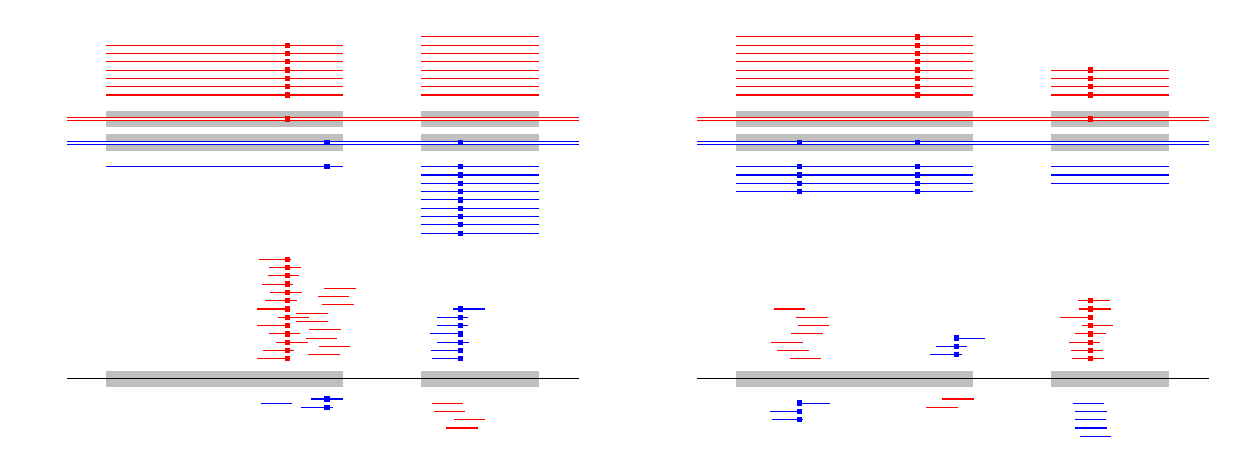
\begin{tikzpicture}[
% SNP variants
var/.style={minimum width=1.5pt, minimum height=1.5pt, inner sep=0, thin, rectangle},
altvar/.style={var, draw, fill},
refvar/.style={var},
% RNA or DNA molecules
DNA/.style={},
matDNA/.style={DNA, red, double},
patDNA/.style={DNA, blue, double},
% RNA-seq reads
read/.style={},
matread/.style={read, red},
patread/.style={read, blue},
% genes (ORFs)
orf/.style={fill=lightgray, very thin}
]

\pgfmathsetseed{1976}

%\draw[very thin, color=gray] (0,0) grid (16,6);

% genome 1 start
\coordinate (g1start) at (0.5,0);
% genome 1, gene 1 and its SNPs
\coordinate (g1g1start) at (1,0);
\coordinate (g1g1s1) at (1.8,0);
\coordinate (g1g1s2) at (3.3,0);
\coordinate (g1g1s3) at (3.8,0);
\coordinate (g1g1end) at (4,0);
% genome 1, gene 2 and its SNPs
\coordinate (g1g2start) at (5,0);
\coordinate (g1g2s1) at (5.5,0);
\coordinate (g1g2end) at (6.5,0);
% genome 1 end
\coordinate (g1end) at (7,0);

% genome2
\path let \n1 = {8} in
(g1start) +(\n1,0) coordinate (g2start)
(g1g1start) +(\n1,0) coordinate (g2g1start)
(g1g1s1) +(\n1,0) coordinate (g2g1s1)
(g1g1s2) +(\n1,0) coordinate (g2g1s2)
(g1g1s3) +(\n1,0) coordinate (g2g1s3)
(g1g1end) +(\n1,0) coordinate (g2g1end)
(g1g2start) +(\n1,0) coordinate (g2g2start)
(g1g2s1) +(\n1,0) coordinate (g2g2s1)
(g1g2end) +(\n1,0) coordinate (g2g2end)
(g1end) +(\n1,0) coordinate (g2end)
;

% draw genome 1

\genomeone{matDNA}{3.3}{}{altvar}{}{}
\genomeone{patDNA}{3}{}{}{altvar}{altvar}

\matRNAgenomeone{3.5}{}{altvar}{}{}{7}{8}
\patRNAgenomeone{2.8}{}{}{altvar}{altvar}{1}{9}

\genomeone{DNA}{0}{}{}{}{}

\mappedreads{g1g1s2}{13}{+}{-}{matread}{altvar}
\mappedreads{g1g1s2}{1}{-}{-}{patread}{}

\mappedreads{g1g1s3}{9}{+}{+}{matread}{}
\mappedreads{g1g1s3}{2}{-}{+}{patread}{altvar}

\mappedreads{g1g2s1}{7}{+}{-}{patread}{altvar}
\mappedreads{g1g2s1}{4}{-}{-}{matread}{}



% draw genome 2

\genometwo{matDNA}{3.3}{}{}{}{altvar}
\genometwo{patDNA}{3}{altvar}{altvar}{}{}
\genometwo{DNA}{0}{}{}{}{}

\matRNAgenometwo{3.5}{}{altvar}{}{altvar}{8}{4}
\patRNAgenometwo{2.8}{altvar}{altvar}{}{}{4}{3}

\mappedreads{g2g1s1}{7}{+}{-}{matread}{}
\mappedreads{g2g1s1}{3}{-}{-}{patread}{altvar}

\mappedreads{g2g1s3}{3}{+}{+}{patread}{altvar}
\mappedreads{g2g1s3}{2}{-}{+}{matread}{}

\mappedreads{g2g2s1}{8}{+}{-}{matread}{altvar}
\mappedreads{g2g2s1}{5}{-}{-}{patread}{}



\end{tikzpicture}
\end{document}
